\documentclass{beamer}
\usetheme{Madrid}
\usecolortheme{beaver}
\usepackage{textpos}

\title{TRIUMF nEXO SiPM Studies}
\author[]{
\includegraphics[height=2.0cm,width=2.2cm]{./EXO.png}\\ \vspace{0.5cm} \\Fabrice Reti\`{e}re\\Carl Rethmeier\\Lloyd James\\Paul Lopes Gomes\vspace{-0.5cm}}
\institute[]{
\includegraphics[height=0.8cm,width=2.5cm]{./TRIUMF.png}}
\date{\today}

\setbeamertemplate{footline}
{
  \leavevmode%
  \hbox{%
  \begin{beamercolorbox}[wd=.333333\paperwidth,ht=2.25ex,dp=1ex,right]{author in foot/foot}%
    \usebeamerfont{author in foot/foot}\insertshortauthor%~~\beamer@ifempty{\insertshortinstitute}{}{(\insertshortinstitute)}
  \end{beamercolorbox}%
  \begin{beamercolorbox}[wd=.333333\paperwidth,ht=2.25ex,dp=1ex,center]{title in foot/foot}%
    \usebeamerfont{title in foot/foot}\insertshorttitle
  \end{beamercolorbox}%
  \begin{beamercolorbox}[wd=.333333\paperwidth,ht=2.25ex,dp=1ex,right]{date in foot/head}%
    \usebeamerfont{date in foot/head}\insertshortdate{}\hspace*{2em}
    \insertframenumber{} / \inserttotalframenumber\hspace*{2ex} 
  \end{beamercolorbox}}%
  \vskip0pt%
}
\makeatother


\begin{document}

\begin{frame}
\maketitle
\end{frame}

\addtobeamertemplate{frametitle}{}{%
\begin{textblock*}{100mm}(.85\textwidth,-1cm)
\vspace{0.5mm}
\hspace{-2.5cm}

\includegraphics[height=0.8cm,width=2.5cm]{./TRIUMF.png}
\hspace{0.5cm}

\includegraphics[height=0.9cm,width=0.9cm]{./EXO.png}
\end{textblock*}}

\begin{frame}{VUV3 Breakdown Voltage}
\begin{figure}
\centering
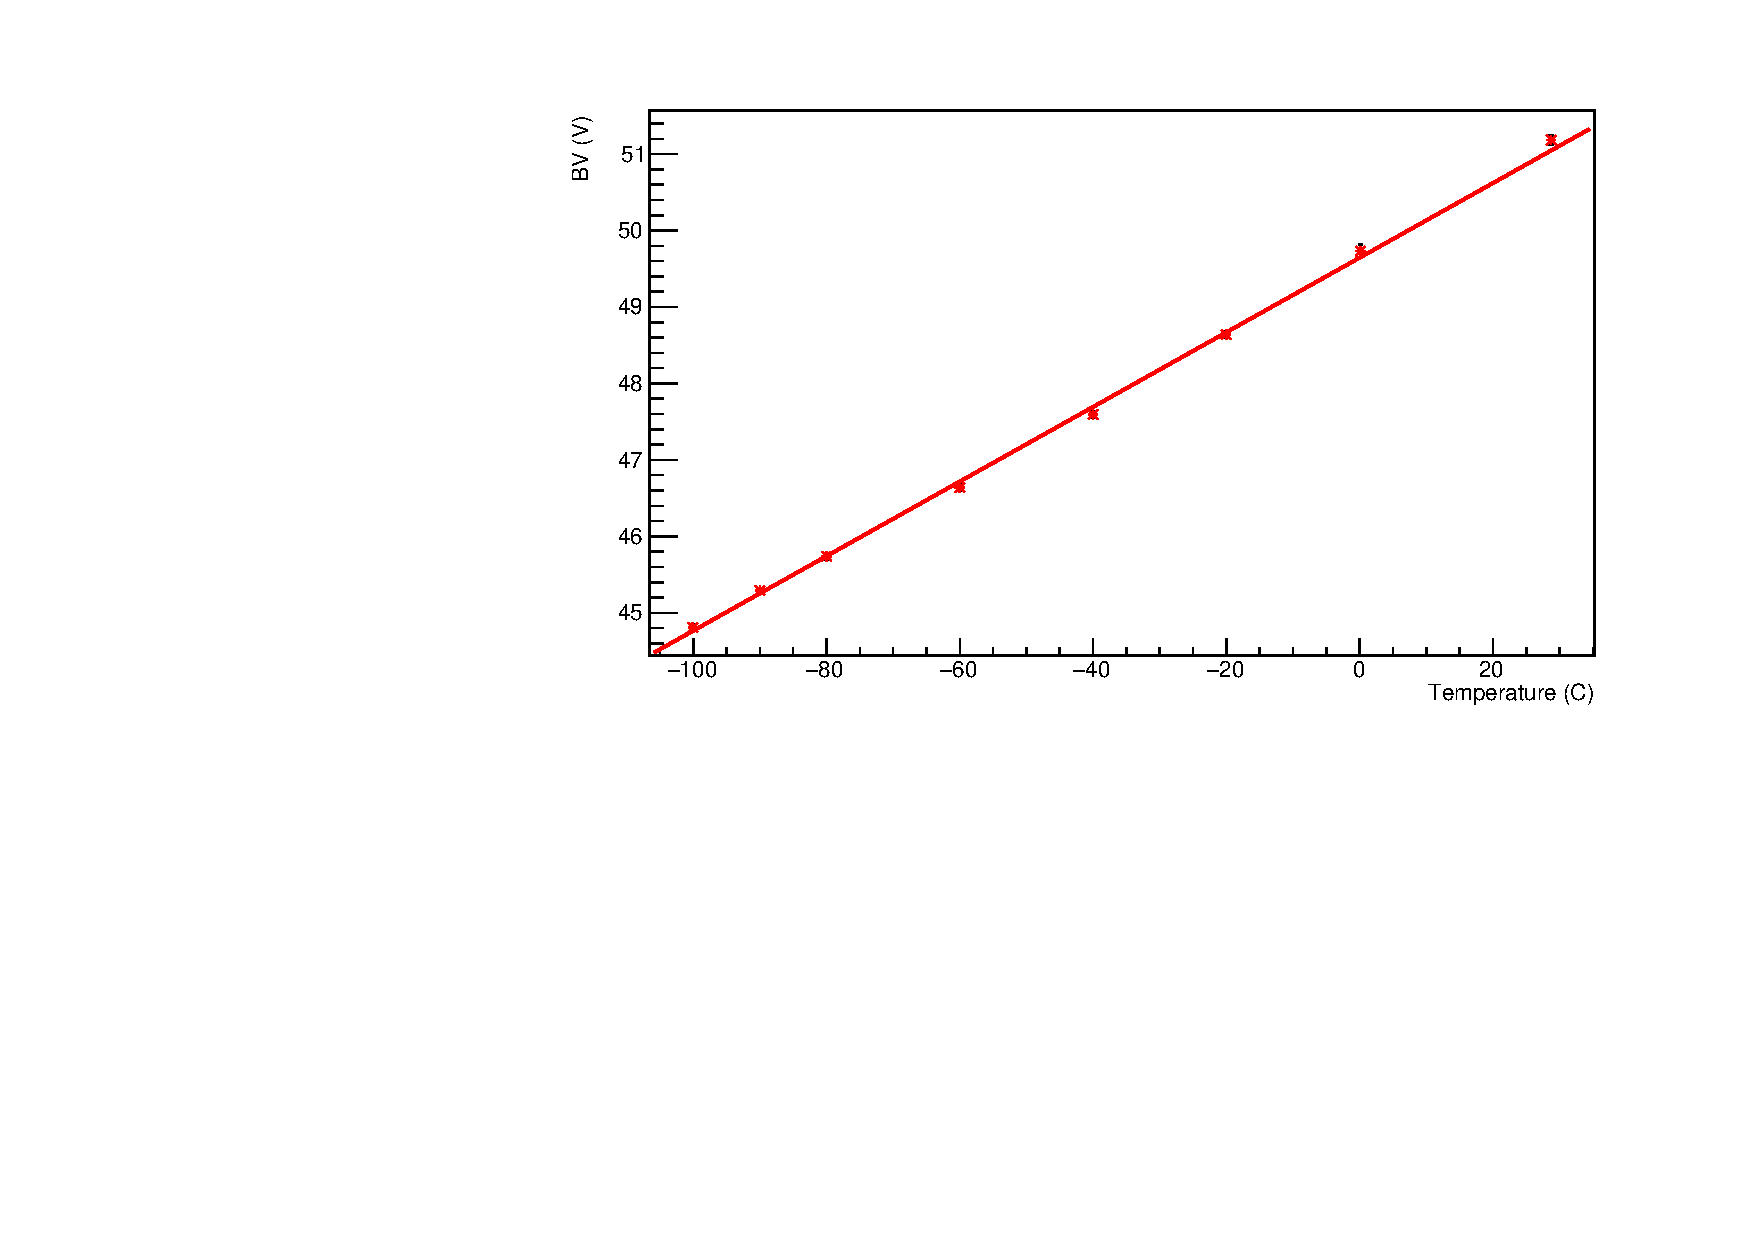
\includegraphics[height=0.5\textwidth]{Gain_Temperature.pdf}
\caption{Breakdown Voltage against Temperature for VUV3 device.}
\end{figure}
\end{frame}

\begin{frame}{Cross-talk}
\begin{figure}
\centering
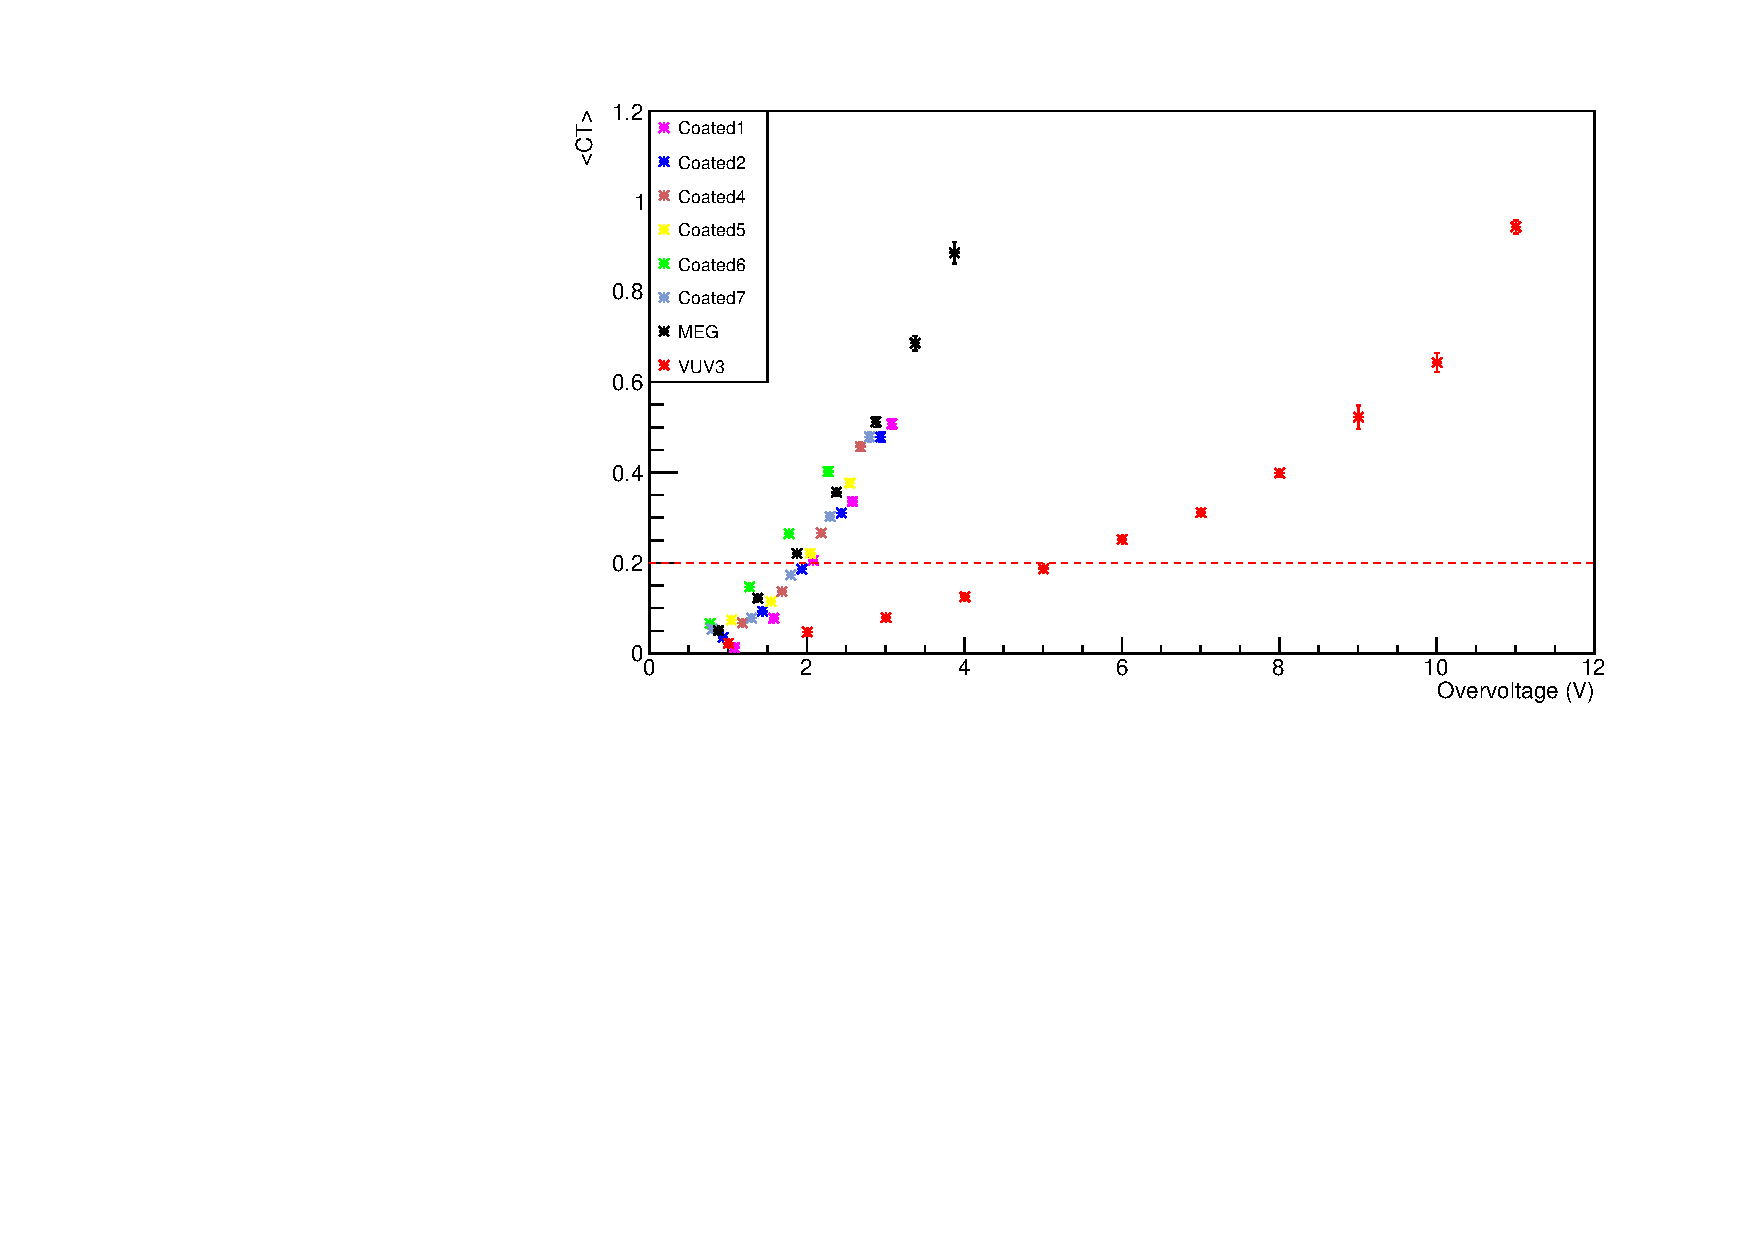
\includegraphics[height=0.5\textwidth]{CTAug7.pdf}
\caption{Crosstalk rate against overvoltage for different devices.}
\end{figure}
\end{frame}

\begin{frame}{Delta-t Distribution}
\begin{figure}
\centering
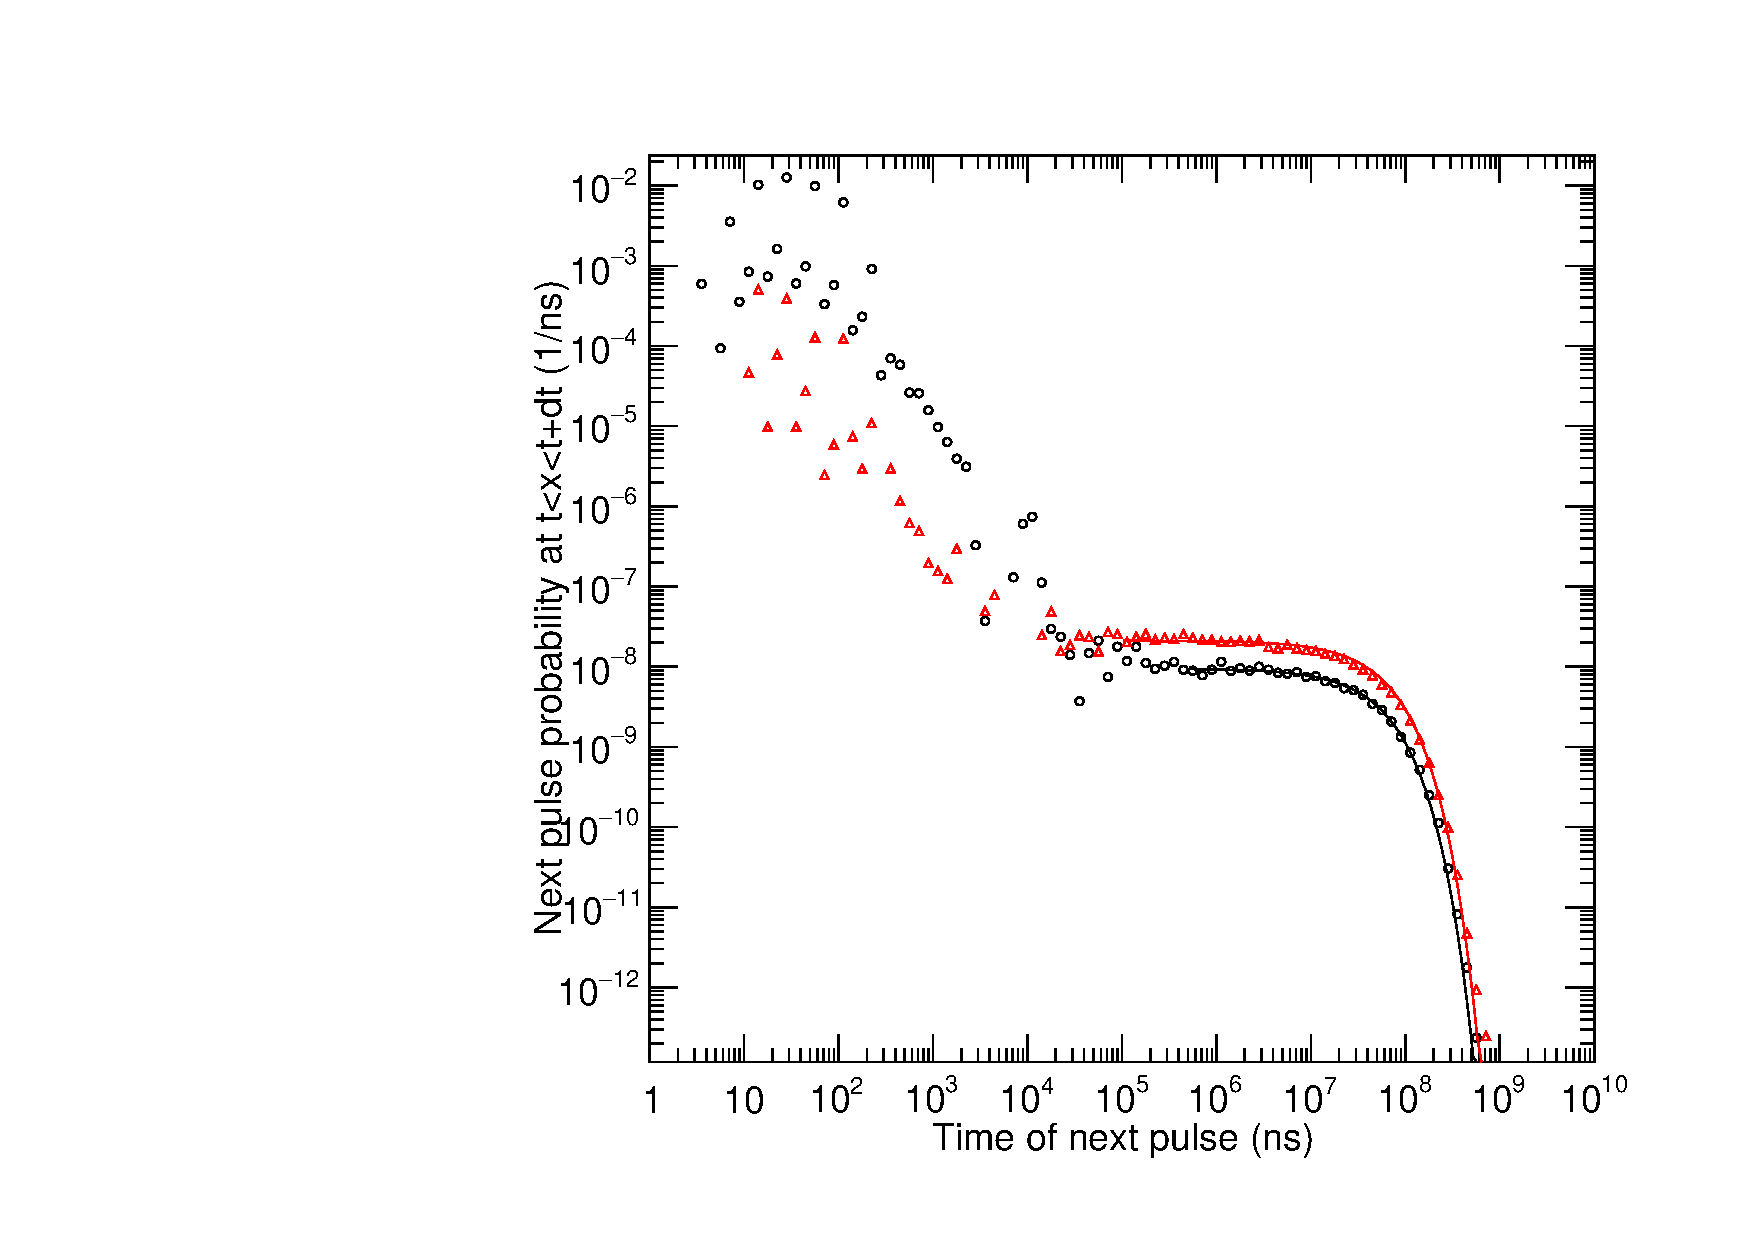
\includegraphics[height=0.5\textwidth]{DTVUV3.pdf}
\caption{Delta-time distribution for VUV3 device. Fit params are : 49.72V - prob. 0 AP = 1; dark rate = 25.3Hz. 57.72V - prob. 0 AP = 0.48; dark rate = 173Hz.}
\end{figure}
\end{frame}

\begin{frame}{Pulse Amplitude vs Time - VUV3}
\begin{figure}
\centering
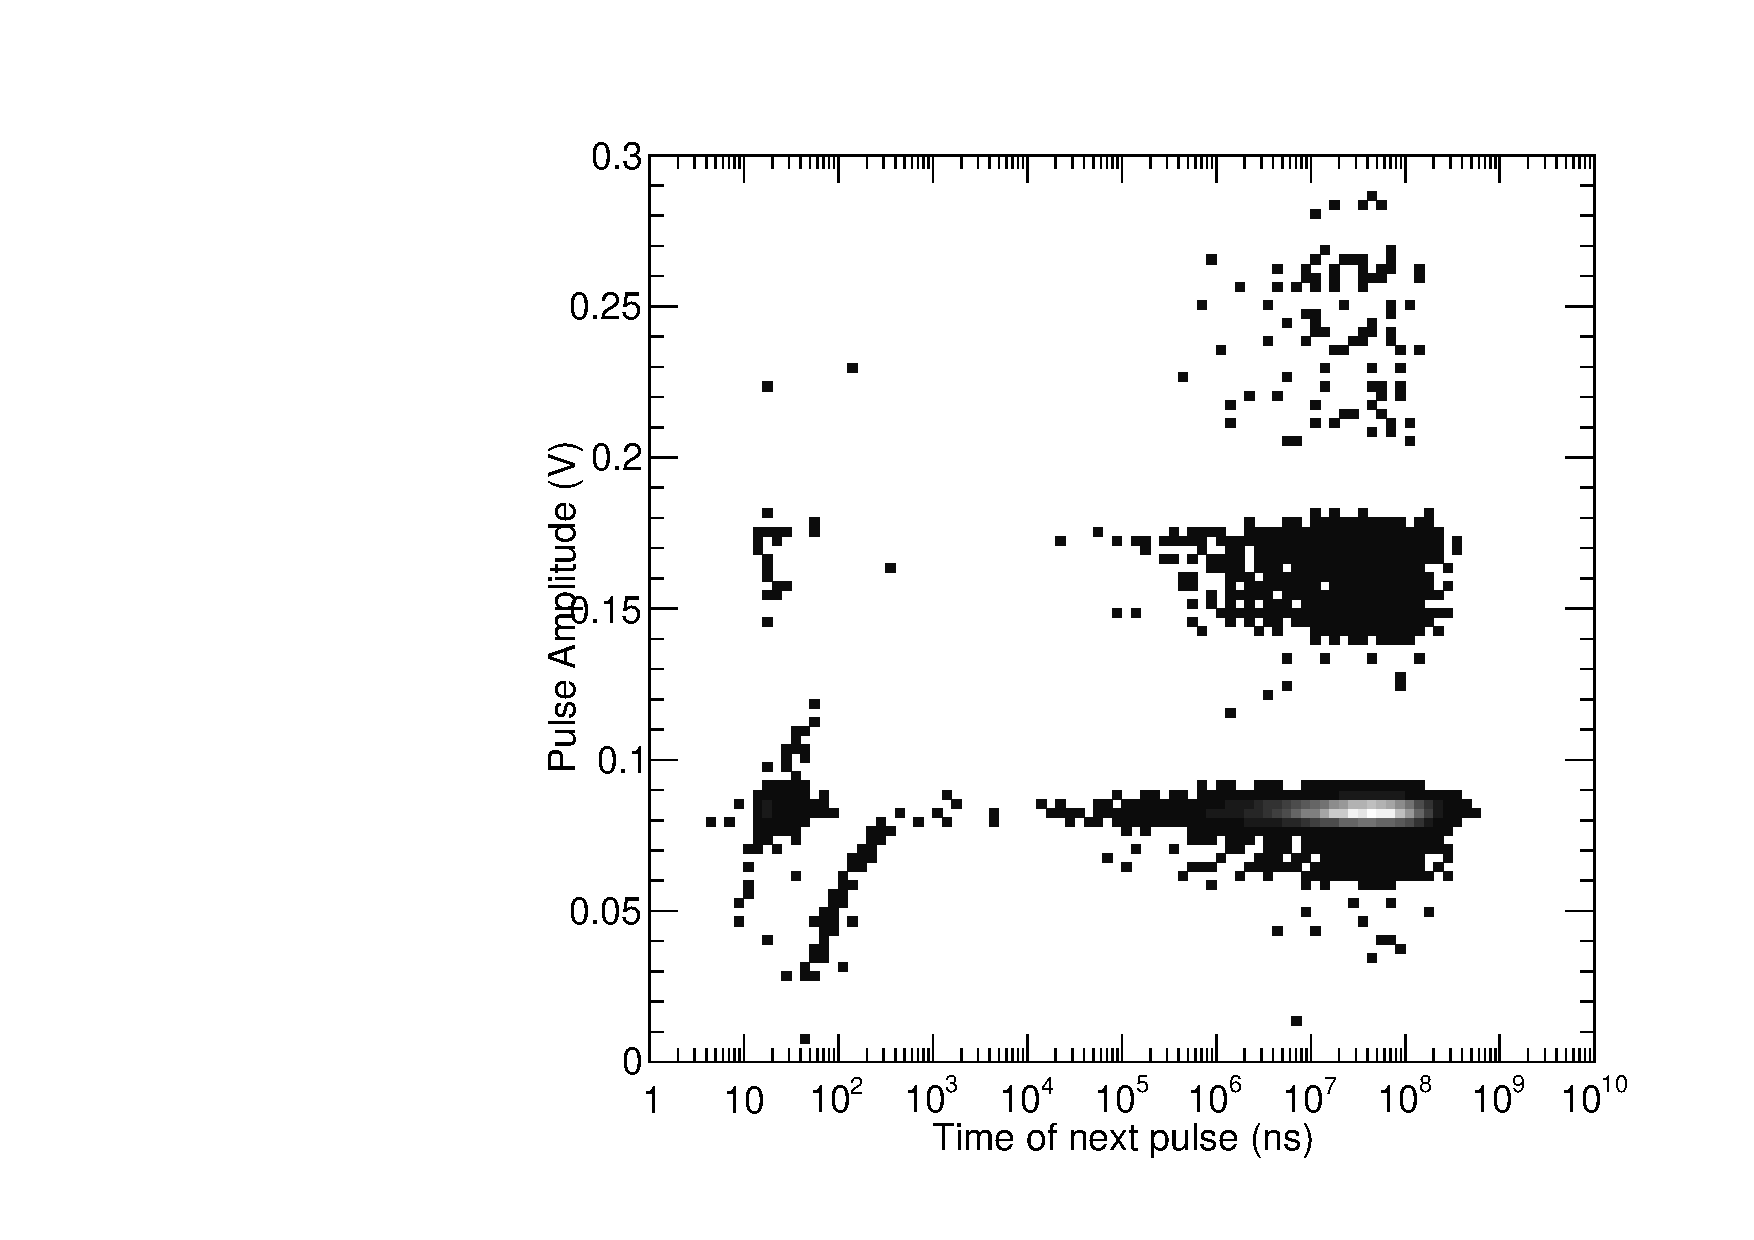
\includegraphics[height=0.5\textwidth]{AmpVUV3.pdf}
\caption{Amplitude of pulses against the time between the pulse and the previous pulse.}
\end{figure}
\end{frame}

\begin{frame}{Light Leak}
\begin{figure}
\centering
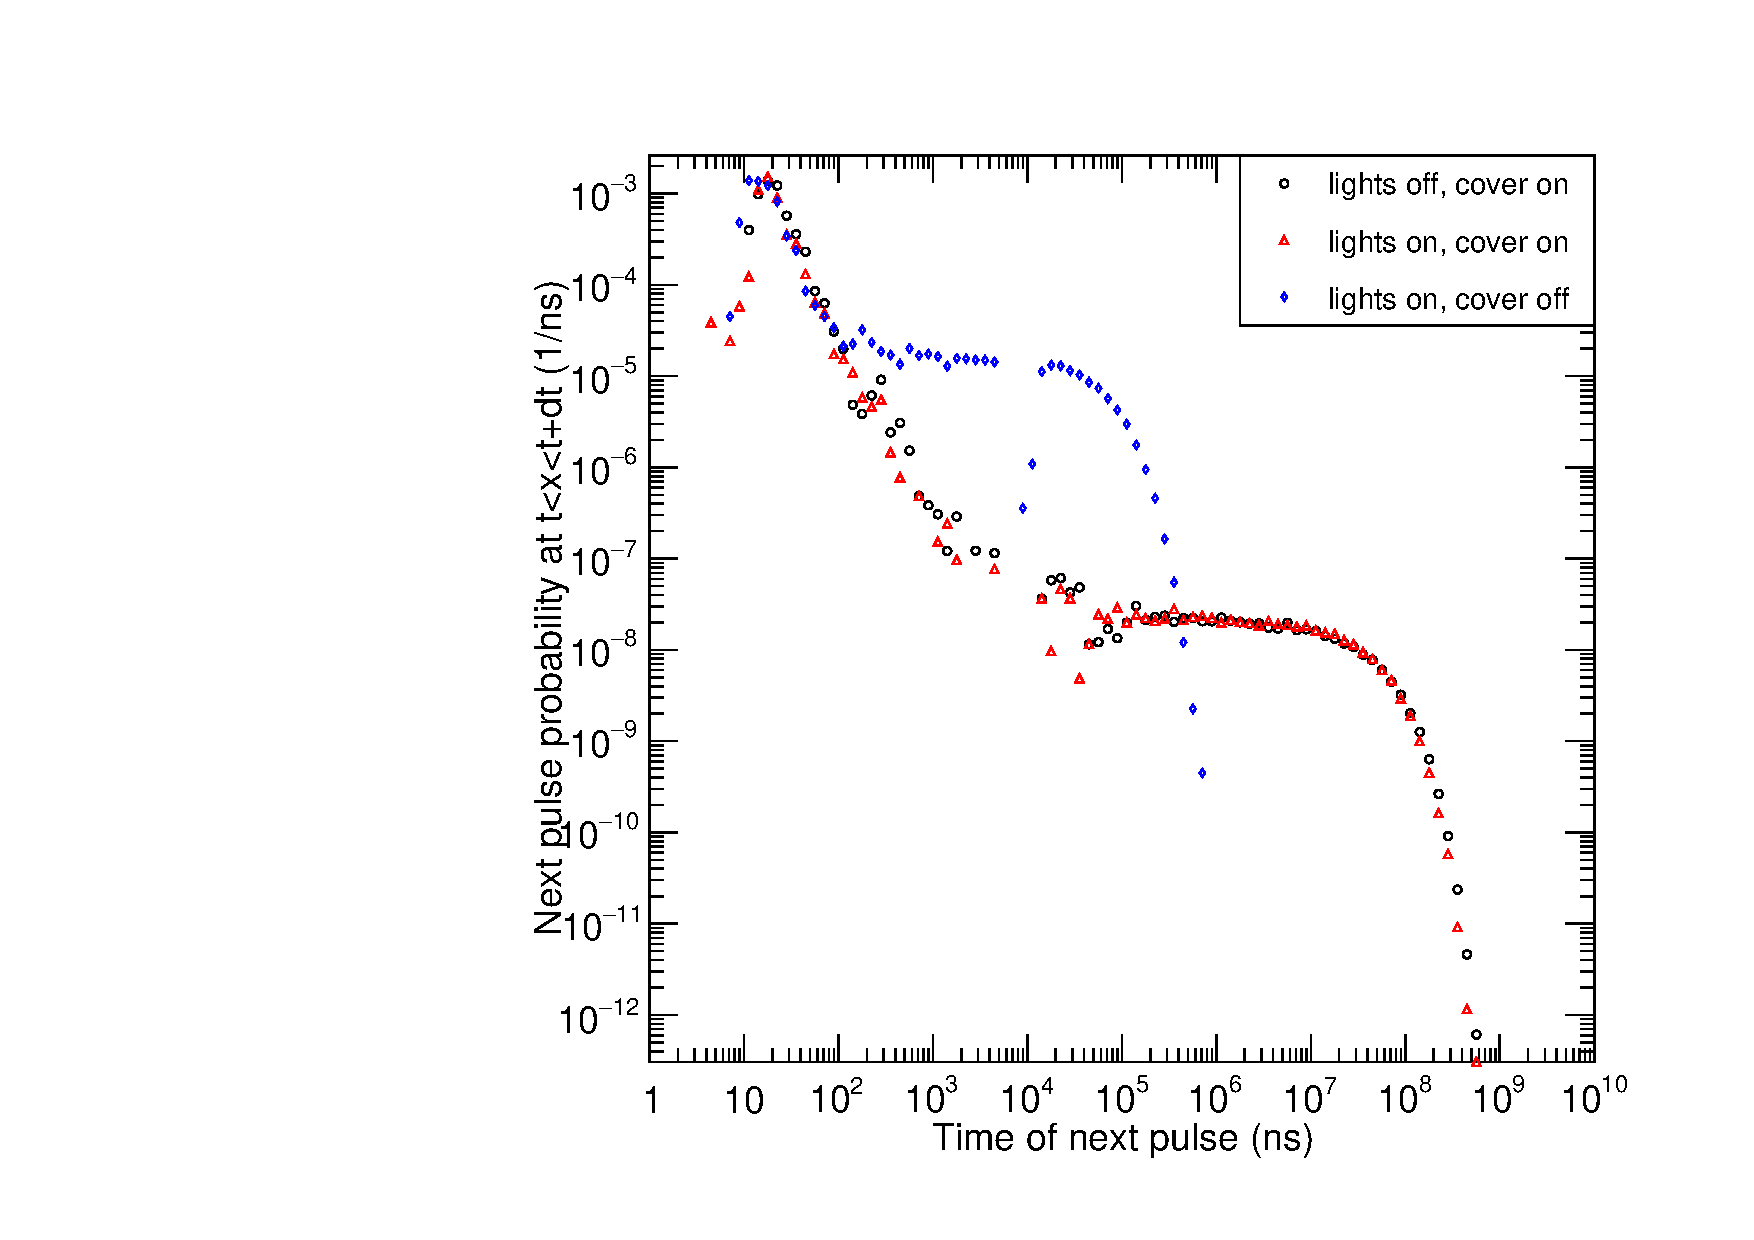
\includegraphics[height=0.5\textwidth]{LightLeak.pdf}
\caption{Delta-time distribution showing that while there is light leak into the box, with the steps taken to cover the box there is no longer a leak.}
\end{figure}
\end{frame}

\begin{frame}{Troubleshooting}
In determining the source of the inconsistency in PE measurements:\\
\begin{itemize}
\item It was determined that cooling was a factor, and we proceeded to test its connection with the beamsplitter. This was motivated by the anticorrelation has that been observed.
\item Temperature sensors were installed in the setup to keep track of temperature at different places in the box.
\end{itemize}
\end{frame}

\begin{frame}{Temperature Sensors}
\begin{figure}
\centering
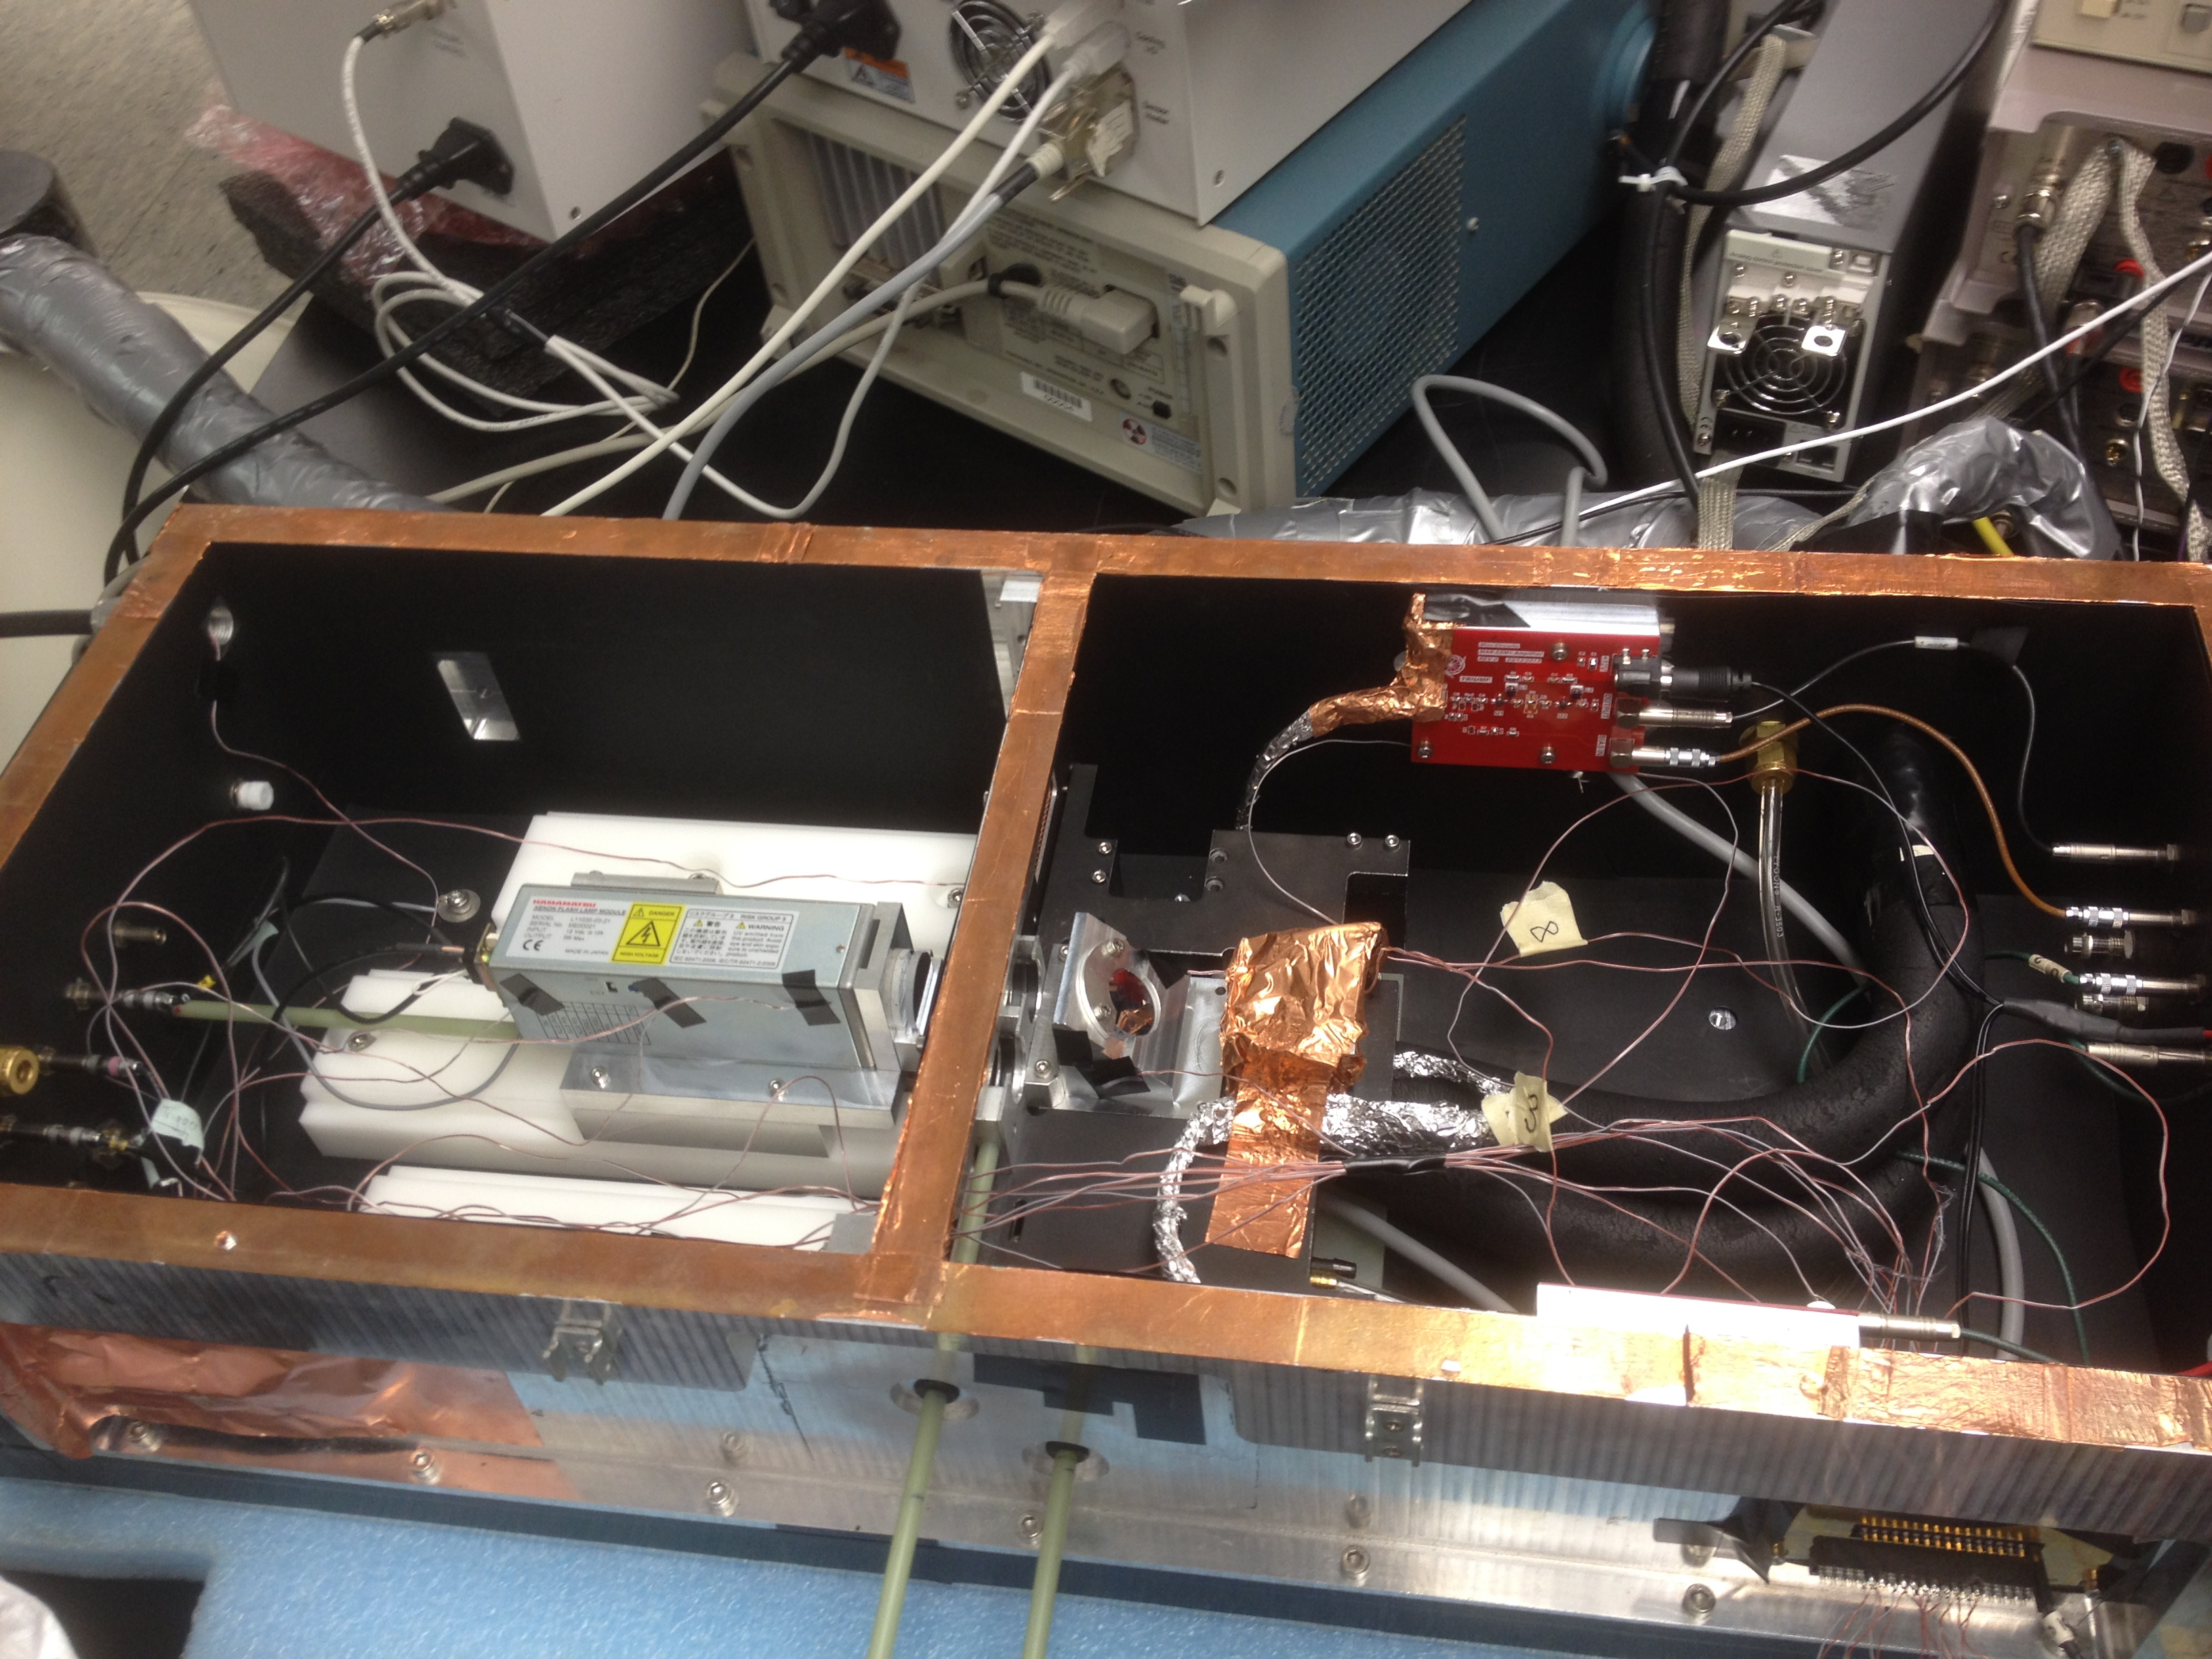
\includegraphics[height=0.5\textwidth]{sensors.JPG}
\caption{10 thermocouples were installed in various locations around the box so that temperature could be recorded in each location over time.}
\end{figure}
\end{frame}

\begin{frame}{Lamp Troubleshooting}
\begin{figure}
\centering
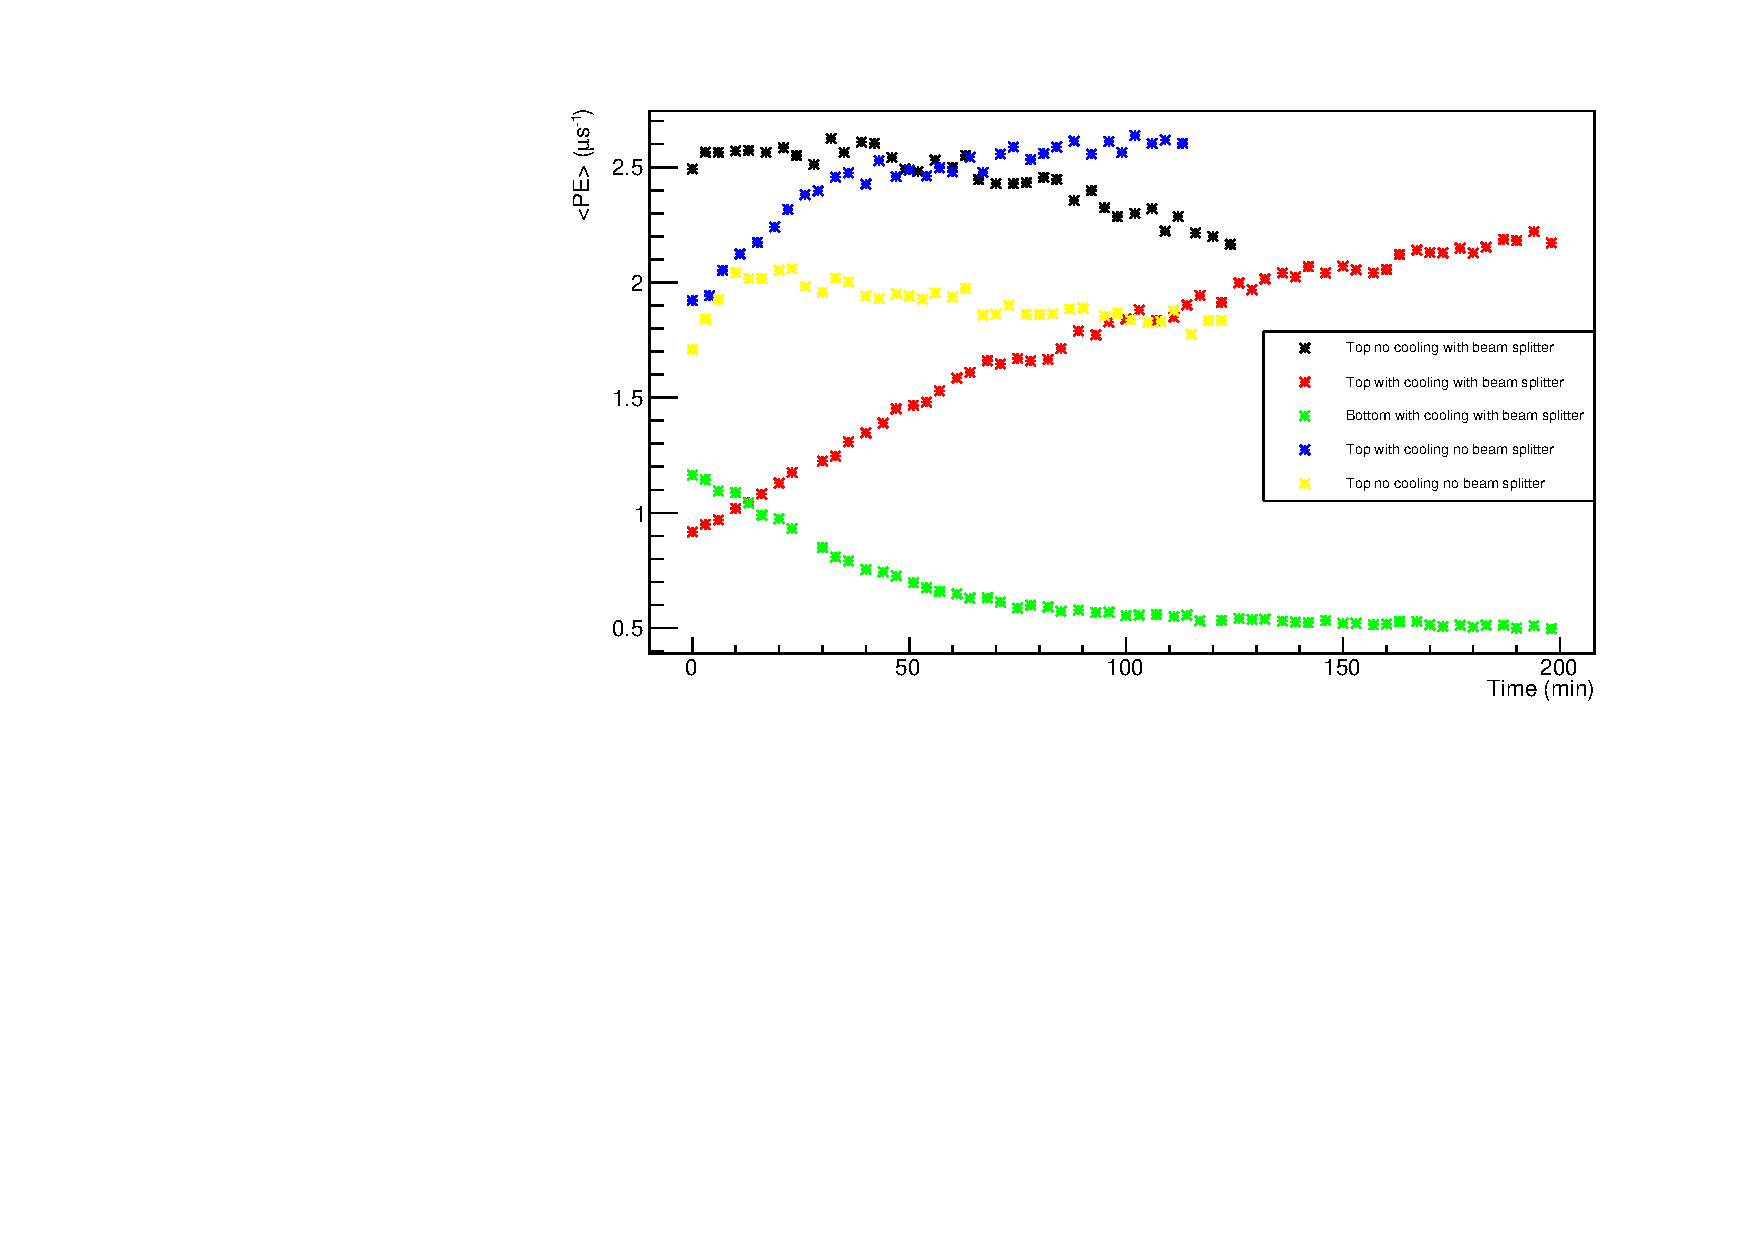
\includegraphics[height=0.5\textwidth]{NewLampPEAug5.pdf}
\caption{PE variation over 200 minutes in different cooling conditions.}
\end{figure}
\end{frame}

\begin{frame}{Lamp Troubleshooting}
\begin{figure}
\centering
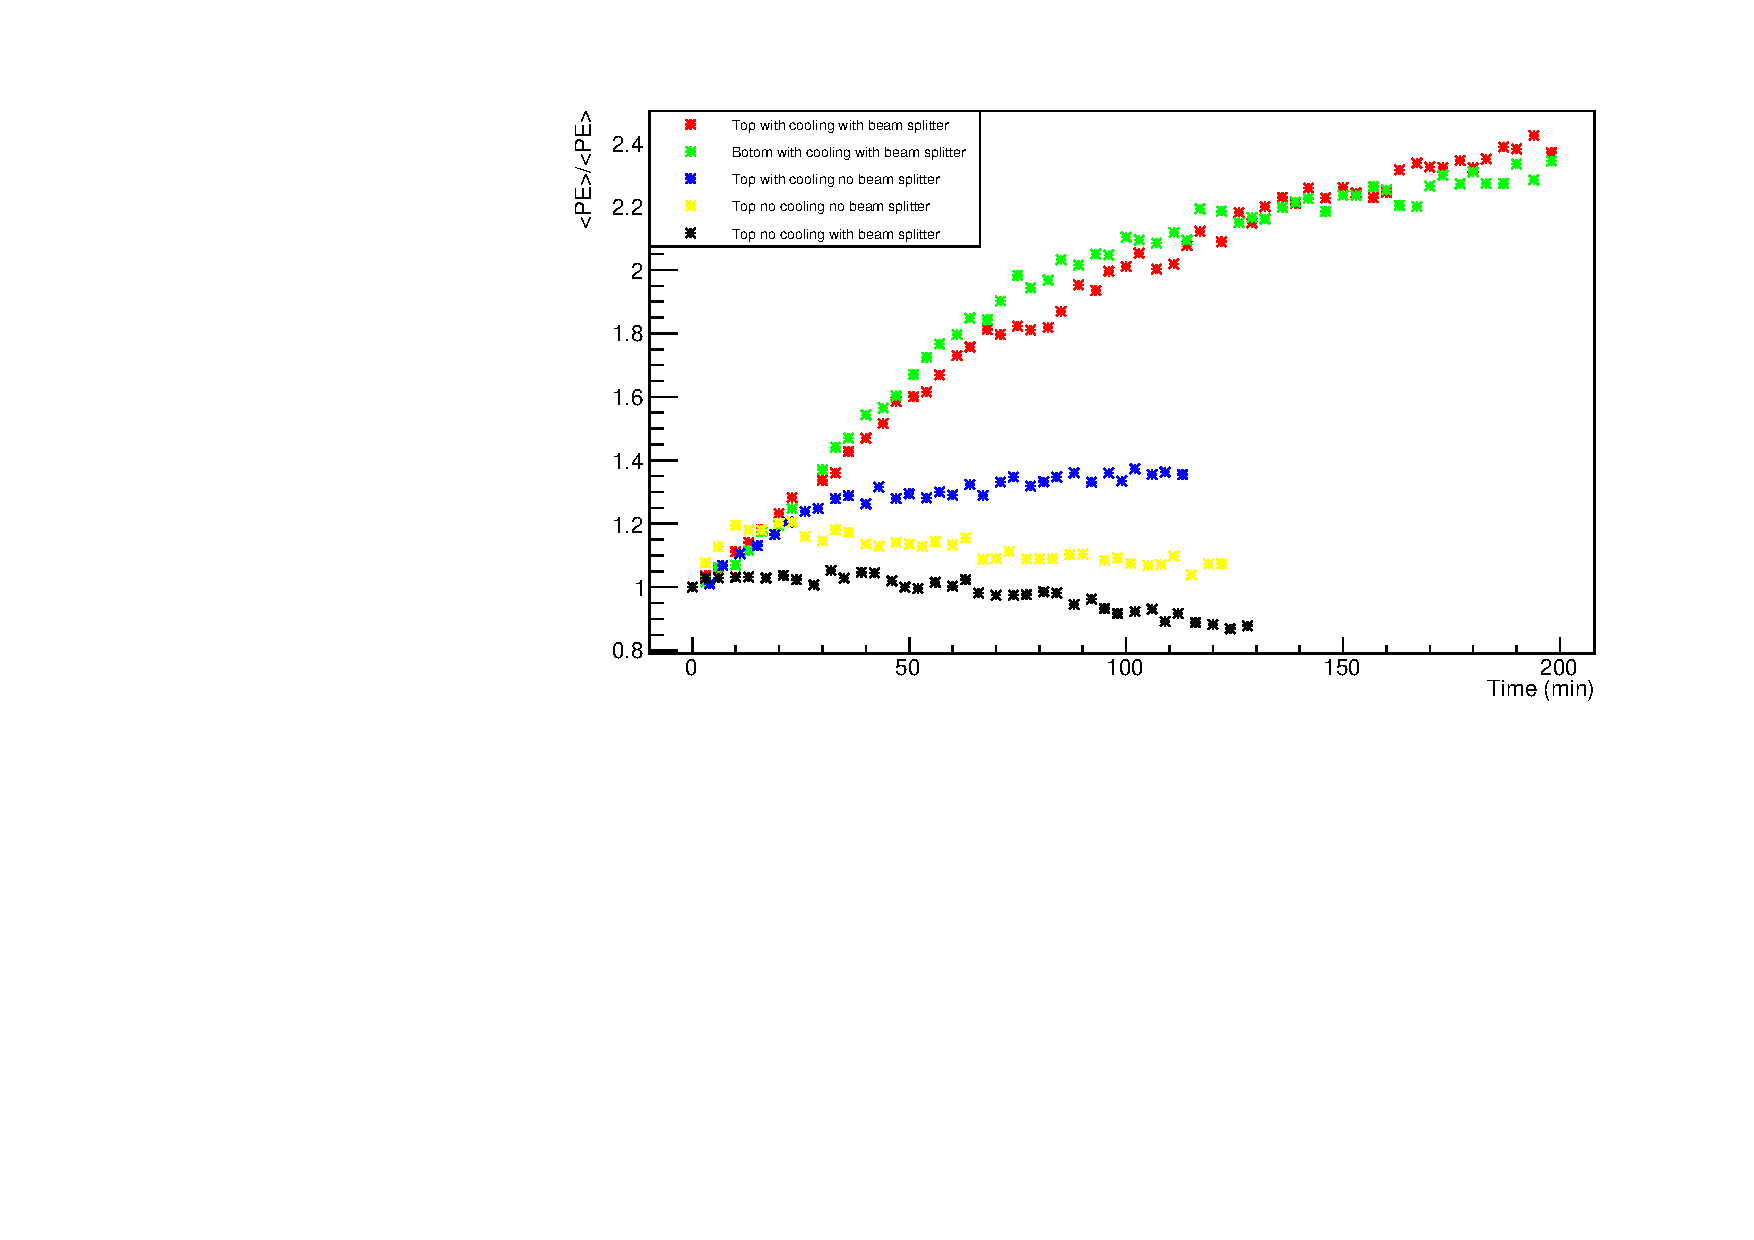
\includegraphics[height=0.5\textwidth]{NewLampPERatioAug10.pdf}
\caption{Variation of ratio of PE to initial PE over 200 minutes in different cooling conditions.}
\end{figure}
\end{frame}

\begin{frame}{Automation}
\begin{itemize}
\item Remote control of the power supply / picoammeter was implemented and interfaced with the scope DAQ software so that voltage scans can now be done automatically. 
\item Remote reading of temperature data from the 10 thermocouples was implemented so that temperature throughout the box can be continously monitored and recorded.
\end{itemize}
\end{frame}

\end{document}